

The design, development, and evaluation processes undertaken throughout this thesis have established a functional foundation for visual exploration of synthetic neighborhood explanations and surrogate model structures. The comparative analyses presented in previous sections positioned the thesis system within the landscape of visual analytics for eXplainable AI, identifying both distinctive contributions and opportunities for enhancement. This section examines potential future developments that could extend the system's capabilities and address limitations. These enhancements regard technical improvements to visualization quality and interaction mechanisms, as well as conceptual extensions expanding the framework's analytical scope. While some enhancements address specific limitations discovered during development, others explore opportunities to incorporate proven patterns from surveyed systems into the synthetic neighborhood exploration paradigm.

The proposed enhancements are organized into three thematic categories reflecting different aspects of system improvement. Enhanced visual encoding and representation strategies focus on increasing information density and providing alternative spatial organizations for tree structures. Adaptive interaction mechanisms and progressive disclosure approaches address complexity management and user-controlled information revelation. Alternative analytical perspectives through clustering explore complementary analysis modes that overstep the class-based coloring paradigm currently employed. Together, these enhancement categories suggest natural evolution directions while maintaining the core principle of bidirectional spatial-symbolic coordination that distinguishes the thesis system's approach to neighborhood-based local explanations.

\subsection{Enhanced Visual Encoding and Representation}

The current system employs established visual encoding strategies including variable-width edges for sample flow, class-based node coloring, and hierarchical node-link layouts. While these encodings prove effective for basic neighborhood exploration workflows, opportunities exist to increase information density and provide alternative spatial organizations that may better support specific analytical tasks. This subsection examines two enhancements focused on visual representation: multi-colored branch encoding inspired by BaobabView's approach, and an alternative horizontal partition layout that emphasizes distributional importance over hierarchical structure.

\subsubsection{Multi-Colored Branch Encoding}

The thesis system currently employs variable-width edges to encode the volume of synthetic instances flowing through each decision branch, with edge color indicating split outcomes (red for negative branches, green for positive branches). While this encoding effectively communicates data flow patterns, each edge segment displays a single uniform color, limiting the identification of class distribution information within branches. Users must rely on tooltip interactions with split nodes to access class distribution statistics, introducing interaction overhead when rapid assessment of class mixing is needed.

Multi-colored edge encoding, following the pattern established by BaobabView \cite{elzen2011baobabview}, would enhance edges by displaying color-coded bands proportional to class distributions within each branch. Each band's width would represent the percentage of instances belonging to a specific class, with total edge width maintaining its current encoding of overall sample flow. This approach would enable immediate visual assessment of class composition at any point in the decision structure without requiring tooltip interactions. For binary and ternary classification tasks, band encoding would provide clear visual feedback about decision boundary quality: branches containing highly mixed class distributions would display wide bands for multiple classes, indicating regions where the surrogate model struggles to achieve clean class separation, while branches with dominant single-class distributions would display narrow bands for minority classes or potentially single-color edges for pure branches.

The analytical value of multi-colored edges becomes particularly apparent when examining synthetic neighborhood quality. Neighborhoods generated by genetic algorithms may exhibit varying degrees of class homogeneity across different decision paths. Edges with pronounced multi-colored banding would immediately reveal decision points where synthetic instances with heterogeneous class distributions coexist, potentially indicating that the neighborhood spans multiple distinct decision regions or that the surrogate model's approximation introduces artificial boundary complexity. Conversely, consistently single-colored edges throughout most branches would provide visual confirmation that the synthetic neighborhood maintains coherent class distributions, suggesting high-quality neighborhood generation and effective surrogate model approximation. This encoding would maintain full compatibility with the existing variable-width encoding approach, as total edge width would continue to represent aggregate sample flow while internal band composition would add distributional detail.

The enhancement introduces trade-offs between information density and visual simplicity. While multi-colored edges would reduce reliance on tooltip interactions for distribution information, they would simultaneously increase visual complexity in ways that may challenge users who prefer cleaner, more minimalist visualizations. The tooltip information revealing precise numerical percentages would become partially redundant with visual band widths, though tooltips would remain valuable for exact quantitative assessment. The multi-colored encoding may also compete visually with existing design elements: split nodes currently employ neutral gray coloring while leaf nodes display class-specific colors, and introducing multi-colored edges throughout the tree might create visual competition between edge bands and node colors. Careful visual hierarchy management through saturation, brightness, or opacity adjustments would be necessary to ensure that critical elements like the explained instance path and leaf node predictions maintain appropriate visual prominence despite increased edge representation complexity.

\subsubsection{Horizontal Partition Chart Alternative Layout}

The three tree layouts currently implemented in the thesis system, Tree Layout, Rule and Counterfactual Rules Centered, and Rule Centered, all employ node-link representations where parent-child relationships appear through explicit edge connections between discrete nodes. While these hierarchical visualizations excel at revealing tree topology and supporting path tracing, they allocate space proportionally to tree structure rather than data importance, treating branches containing thousands of instances identically to branches containing only a few edge cases. This space allocation strategy prioritizes structural comprehension over distributional emphasis, potentially obscuring which decision paths capture the majority of the synthetic neighborhood.

A horizontal partition chart layout, shown in Figure \ref{fig:altTreeLayout}, would introduce a fundamentally different spatial organization based on proportional space filling rather than topological node positioning. This layout would represent the root node as a horizontal bar spanning the full width of the visualization, with bar width encoding the total percentage of synthetic instances (100\% at the root). Each decision split would partition the parent bar into vertically stacked child segments, with segment widths proportional to the percentage of instances flowing through each branch. Tree depth would progress horizontally from left to right, with split points creating vertical divisions and leaf nodes appearing as rightmost bar segments colored according to predicted classes. This representation would sacrifice the explicit edge connections of node-link diagrams in favor of immediate distributional visibility through spatial area allocation.

\begin{figure}
    \centering
    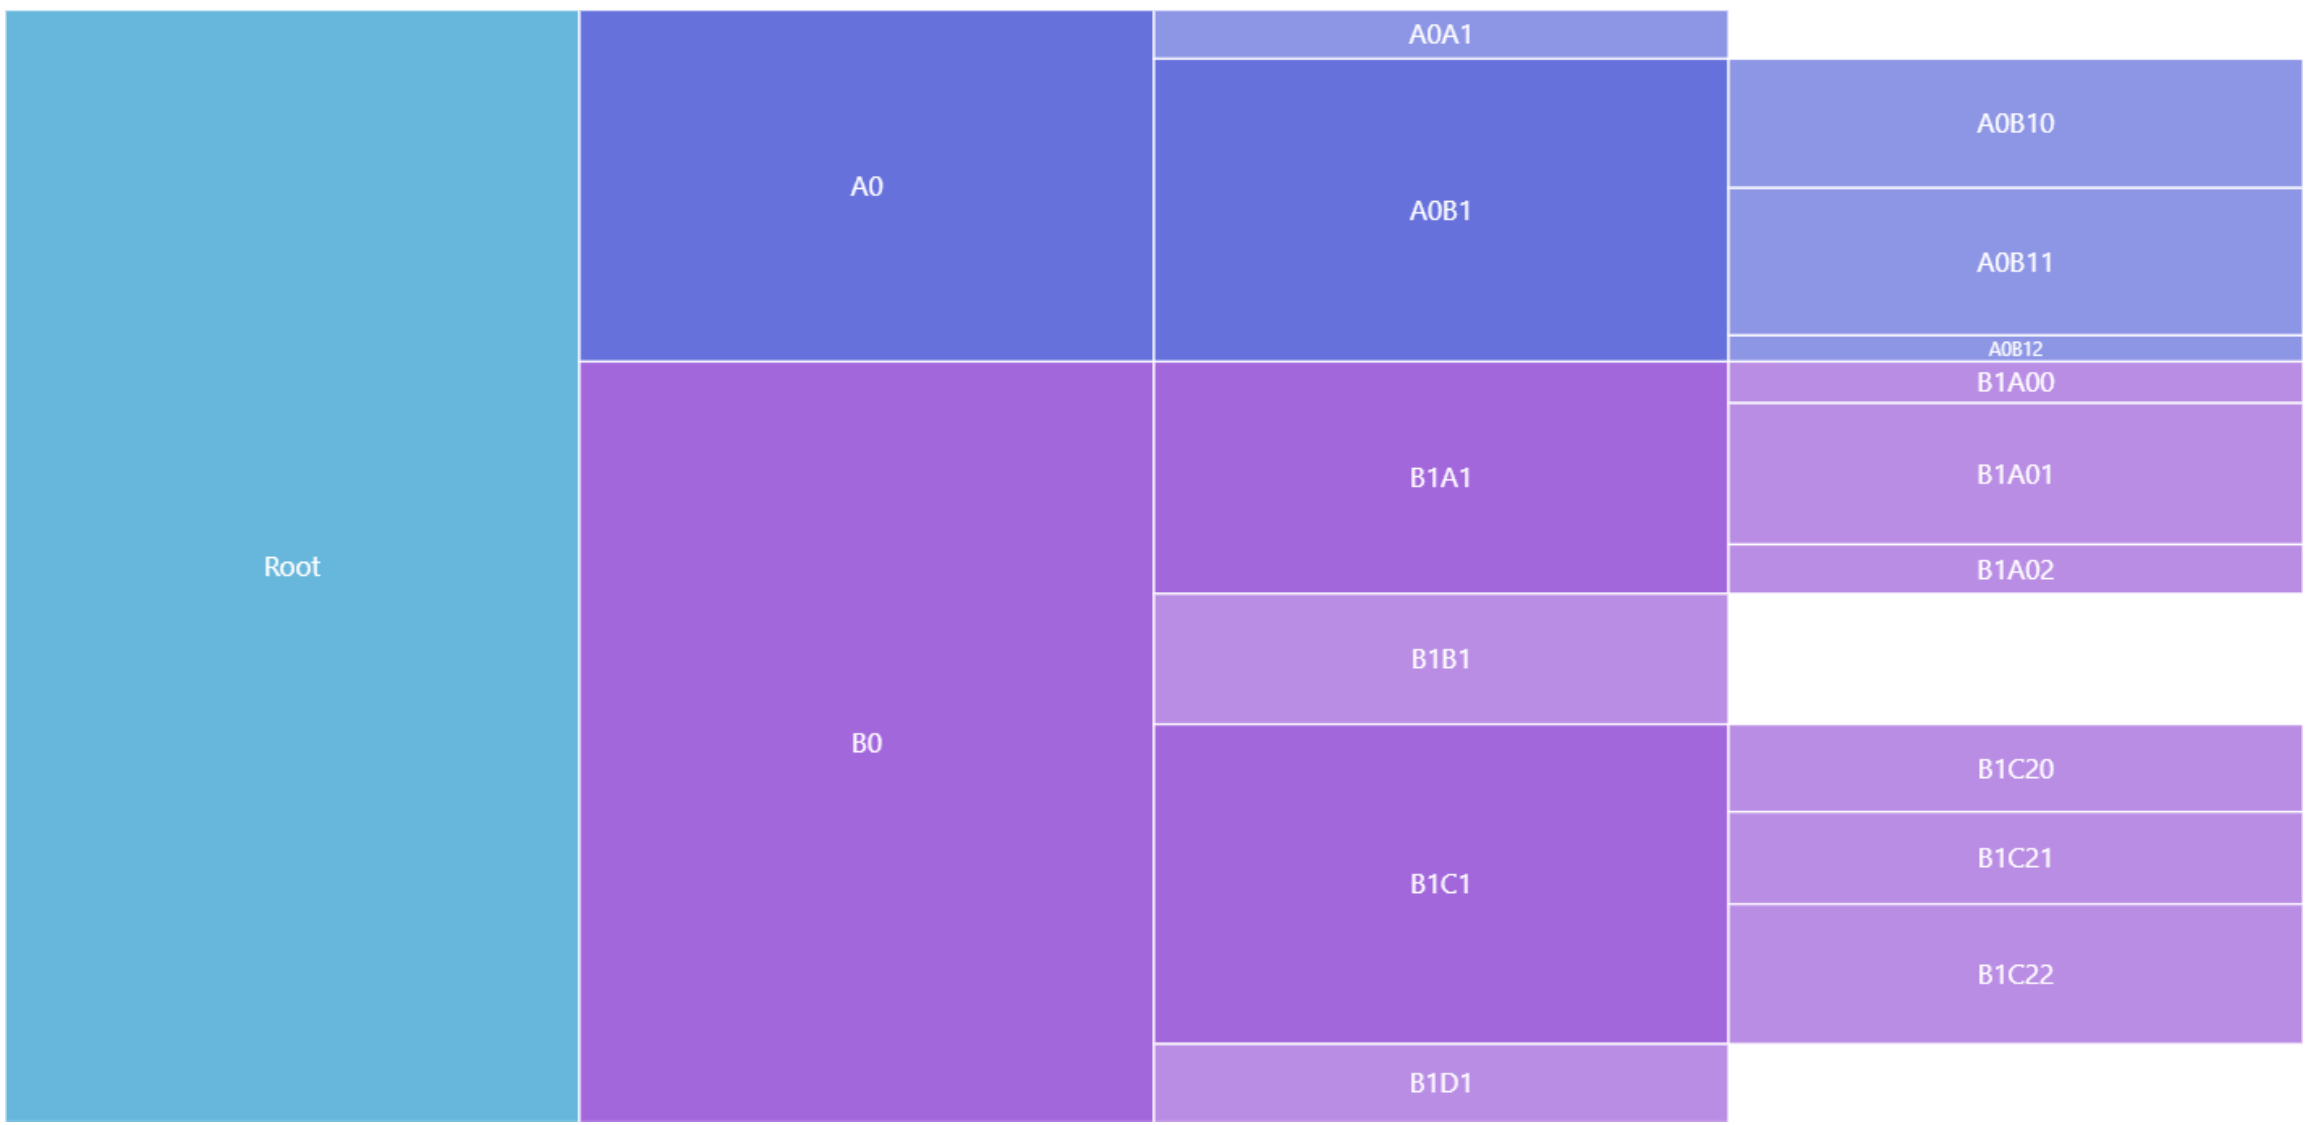
\includegraphics[width=0.8\linewidth]{images/alternative Tree Layout.png}
    \caption{Concept of the alternative tree layout proposed, extracted from \cite{horizontalPartitionChart}}
    \label{fig:altTreeLayout}
\end{figure}

The analytical benefits of this alternative layout become apparent when considering common neighborhood exploration workflows. Users frequently need to identify which decision paths contain the majority of synthetic instances to identify the rules and the counterfactual rules found by the explainability method. In the current node-link layouts, identifying dominant paths is performed by the users by the 
deciphering edge widths across multiple levels or examining the sample count inside the tooltips. The horizontal partition layout would make path importance immediately visible through bar width: paths containing 60\% of neighborhood instances would occupy 60\% of the horizontal space, while paths with only 2\% would appear as narrow slivers. This proportional space allocation would enable rapid identification of the most significant decision patterns without requiring interaction or mental aggregation. Terminal bar segments representing leaf nodes would provide an immediate overview of final prediction distributions, with segment widths revealing the relative populations of different predicted classes and segment heights indicating how many distinct decision paths lead to each class prediction. Compact representation of deep trees would emerge naturally, as depth progression occurs horizontally rather than vertically, potentially enabling more efficient space utilization for trees with substantial depth but limited branching factors at most levels.

However, this alternative layout introduces significant limitations alongside its distributional clarity benefits. Path highlighting presents a fundamental challenge: in node-link layouts, highlighting the explained instance path requires merely emphasizing specific nodes and edges, with the hierarchical structure providing inherent visual guidance for path following. In the horizontal partition layout, identifying specific instance paths becomes considerably more difficult, as individual instances do not correspond to discrete visual elements but rather contribute fractionally to bar segment populations. Emphasizing a single path might require overlaying transparent highlighting bands that span specific vertical ranges at each horizontal level, but such highlighting could create visual ambiguity about precise path boundaries, particularly when multiple paths diverge and reconverge at different depths. Counterfactual path comparison, one of the core analytical workflows supported by the Rule and Counterfactual Rules Centered layout, would face similar challenges: comparing decision paths at equivalent depths becomes substantially harder when paths appear as vertically stacked segments rather than horizontally aligned rectangular nodes with explicit depth-level positioning. The reduced hierarchical clarity represents another trade-off: while experienced users might adapt to interpreting parent-child relationships through horizontal progression and vertical partitioning, the cognitive load for understanding tree topology would likely increase compared to explicit node-link connections. New users examining their first neighborhood explanation might struggle to understand how the horizontal partition structure encodes the same logical decision tree visible in the traditional layouts.

Integration with the existing thesis system architecture would position the horizontal partition layout as a fourth option in the layout selector, maintaining consistency with the multi-layout paradigm while extending representational alternatives. Color consistency with other layouts should be preserved: bar segments representing leaf predictions would employ the same class-based coloring used for leaf nodes in node-link layouts, and background segments representing internal splits might employ the same neutral gray coloring used for split nodes. 
This enhancement might work most effectively as an initial overview tool where users examine overall neighborhood distribution patterns before switching to node-link layouts for detailed path examination and counterfactual comparison. The horizontal partition layout could serve as an entry point for analysis, helping users quickly identify whether neighborhoods exhibit concentrated distributions dominated by a few major paths or diffuse distributions spread across many alternatives, after which users would transition to Rule Centered or Rule and Counterfactual Rules Centered layouts for focused exploration of specific decision logic.

\subsection{Adaptive Interaction Mechanisms and Progressive Disclosure}

The current system provides multiple tree layouts addressing different analytical priorities but requires full layout switching to transition between Rule Centered's focused representation and Rule and Counterfactual Rules Centered's comparison capabilities. While Rule Centered implements progressive disclosure through collapsible subtrees, the layout switching mechanism operates at coarse granularity, forcing users to choose between complete layout alternatives rather than progressively adjusting information density within a single layout. This subsection examines two enhancements focused on user-controlled complexity management: a hybrid visualization mode enabling incremental transformation between focused and comparative layouts, and threshold-based leaf filtering that dynamically hides low-population branches to reduce visual clutter in large trees.

\subsubsection{Hybrid Visualization Mode}

Rule Centered and Rule and Counterfactual Rules Centered visualizations serve complementary analytical purposes but currently exist as distinct layouts requiring complete switching to transition between them. Rule Centered excels at focusing attention on the explained instance path by rendering it as prominent rectangular nodes while maintaining contextual awareness of alternative branches through collapsible circular nodes. Rule and Counterfactual Rules Centered excels at facilitating counterfactual comparison through depth-aligned rectangular paths that enable direct visual comparison of decision conditions at equivalent tree depths. Users who wish to combine these strengths, focusing primarily on the explained instance path while selectively comparing specific counterfactuals of interest, must currently maintain mental integration across separate layout examinations or accept the visual density of seeing all counterfactual paths simultaneously in the Rule and Counterfactual Rules Centered default state.

A hybrid visualization mode would enable interactive transformation within the Rule Centered layout, allowing users to progressively convert individual counterfactual paths from the circular representations to rectangular depth-aligned representations on demand. The interaction workflow would begin with the standard Rule Centered layout: the explained instance path appears as rectangular nodes positioned horizontally, while all alternative branches stemming from path decision points remain as collapsible circular nodes positioned above and below the central path. When users identify a specific counterfactual leaf of interest, perhaps by examining the scatter plot and noticing a cluster of instances with different class predictions, they could right-click that leaf node and select "Convert to rectangular path" from a context menu. The system would then convert all nodes along the path from root to the selected leaf into rectangular representations and reposition the converted path using depth-alignment algorithms, placing it above the explained instance path (which would maintain its bottom-anchored position). Converted paths would be sorted vertically based on their divergence points from the explained instance path, with paths diverging earlier appearing higher in the layout. Off-path nodes not belonging to either the explained instance path or any converted counterfactual paths would remain as collapsible circular nodes, maintaining contextual awareness without visual clutter. Users could iteratively convert additional paths, progressively building a comparison view customized to their specific analytical interests rather than being presented with all possible counterfactuals simultaneously.

The analytical benefits of this progressive transformation approach center on cognitive load management and user-driven exploration. Users examining a neighborhood explanation often begin with a focused question: "Why did the model predict class A for this instance?" The initial Rule Centered layout directly addresses this question by displaying the explanation path. As users develop understanding, they may formulate secondary questions: "What would need to change to produce a class B prediction instead?" or "Why do some instances in the scatter plot's clusters receive different predictions?" The hybrid mode would enable users to address these secondary questions by selectively converting relevant counterfactual paths without overwhelming their working memory with all possible alternatives. This progressive counterfactual exploration supports natural analytical workflows where users start with focused examination and gradually expand scope based on discovered patterns. The approach contrasts with Rule and Counterfactual Rules Centered's default presentation of all counterfactual paths, which may overwhelm users with information before they have developed sufficient context to prioritize which comparisons matters the most. 

\subsubsection{Threshold-Based Leaf Filtering}

Surrogate decision tree models generated for synthetic neighborhood explanations frequently produce numerous leaf nodes containing small percentages of total neighborhood instances. These low-population leaves often represent edge cases, boundary artifacts, or rare feature combinations that, while potentially interesting for specialized analysis, contribute visual clutter that obscures major decision patterns. The current system displays complete tree structures regardless of leaf population distributions, treating a leaf containing 45\% of neighborhood instances identically to a leaf containing 0.3\% of instances. This democratic representation strategy prioritizes comprehensive information access but may overwhelm users examining large neighborhoods where genetic algorithms generate thousands of synthetic instances distributed across dozens of terminal leaves. Particularly when surrogate models grow deep with extensive branching, the proliferation of visually indistinguishable small leaves challenges users' ability to identify which decision paths need detailed examination.

This flaw is handled by the dynamic edge sizing, but a threshold-based leaf filtering would introduce a user-adjustable parameter enabling dynamic hiding of leaves falling below a specified sample percentage threshold. The interaction mechanism would employ a slider control positioned in the visualization toolbar, labeled "Minimum leaf size". As users adjust the slider, the visualization would update in real-time, with leaves containing fewer instances than the threshold percentage disappearing from the display. Parent split nodes would remain visible even when all or most of their children are filtered, creating "stub" branches that indicate decision points exist but terminate without displaying complete subtrees. Visual indicators such as dashed outlines or special iconography on affected split nodes would communicate that some children are hidden, maintaining user awareness that the visualization represents a filtered view rather than the complete tree structure.

The relationship between threshold-based filtering and the focus+context literature \cite{readingsInformationVi} suggests opportunities for more sophisticated approaches: rather than binary show/hide filtering, the system could implement semantic zooming where leaves below the threshold appear in reduced size or lower opacity, maintaining contextual awareness while visually emphasizing high-population paths. This approach would mitigate the information loss concern by keeping all leaves technically visible while clearly distinguishing major patterns through visual hierarchy.

\subsection{Alternative Analytical Perspectives Through Clustering}

The current system employs class-based coloring throughout all visualizations, where scatter plot points and leaf nodes display colors corresponding to predicted class labels. This encoding directly supports the primary analytical goal of verifying that spatial proximity in the neighborhood correlates with classification consistency. However, this single-perspective approach limits exploration of alternative organizational patterns that may exist within synthetic neighborhoods. Neighborhoods may exhibit spatial or feature-space structure that does not align perfectly with class boundaries, and instances receiving identical predictions may nonetheless cluster into distinct subgroups based on underlying feature similarities. This subsection examines two enhancements focused on complementary analytical perspectives: clustering-based alternative coloring schemes that reveal structure independent of classification outcomes, and textual rule export functionality that bridges visual analysis with traditional text-based reporting and code implementation workflows.

\subsubsection{Clustering-Based Alternative Coloring}

All current thesis system visualizations employ class-based coloring where colors map to model predictions: instances predicted as class A receive color A, instances predicted as class B receive color B, and so forth. This encoding maintains consistency across the scatter plot and tree visualizations, enabling users to trace instances between spatial and symbolic representations through color matching. While this approach effectively supports verification workflows, as users can confirm that spatially proximate instances receive similar predictions by observing color clustering patterns, it constrains analysis to the classification perspective. The system provides no mechanism for examining whether alternative organizational structures exist within the synthetic neighborhood that might reveal subpopulations, feature-space patterns, or projection artifacts independent of the surrogate model's decision boundaries.

Clustering-based alternative coloring would implement a toggle-based mode enabling users to switch between class-based coloring and clustering-based coloring throughout the interface. The toggle control, implemented as a radio button or switch in the visualization toolbar labeled "Color by: [Class / Clusters]", would trigger immediate re-coloring of all visual elements without changing spatial positions or tree structure. In cluster mode, colors would be assigned based on clustering algorithms applied to the synthetic neighborhood in either the original high-dimensional feature space or the projected two-dimensional space visible in the scatter plot. Users could select among established clustering algorithms including k-means, DBSCAN, or hierarchical clustering through a secondary control. Color assignment would utilize the same colorblind-safe palette employed for class coloring, mapping palette entries to cluster identifiers rather than class labels. The scope of re-coloring would affect both scatter plot points and corresponding leaf nodes in all tree visualizations simultaneously, maintaining the coordination principle that enables cross-visualization instance tracing. Switching between class mode and cluster mode would provide instantaneous visual feedback, allowing users to rapidly alternate perspectives to examine whether clustering structure aligns with or diverges from classification boundaries.

The analytical value of clustering-based coloring emerges through four primary use cases addressing distinct investigation goals. First, cluster-class correspondence verification enables users to examine whether clustering in feature space aligns with classification boundaries. Strong correspondence, where cluster memberships closely match class predictions, would suggest that the surrogate model's decision boundaries align naturally with the intrinsic structure of the synthetic neighborhood, indicating high-quality neighborhood generation and effective model approximation. Conversely, substantial misalignment, where instances clustering together receive different class predictions, would reveal situations where model predictions contradict natural data organization. This misalignment might indicate that the neighborhood spans multiple decision regions, that the genetic algorithm generated instances exploring boundary regions rather than class-homogeneous areas, or that the surrogate model introduces artificial complexity not present in the original black-box classifier's decision logic. Users examining neighborhoods for specific explained instances could assess whether those neighborhoods are "well-behaved" (clear cluster-class correspondence indicating coherent local decision space) or "boundary-crossing" (mixed clusters indicating complex decision topology).

Second, within-class pattern discovery enables identification of subgroups among instances receiving identical predictions. Even when the surrogate model predicts all instances in a particular tree branch as class A, those instances may cluster into two or three distinct groups based on feature similarities invisible to the class-based coloring scheme. Discovering such within-class clusters might reveal that "class A predictions" actually encompass multiple distinct feature configurations both receive the same class prediction despite occupying different feature space regions and clustering separately. This enhanced resolution supports more nuanced understanding of decision patterns and may inform users about the heterogeneity of predictions within specific rules. Users could investigate questions like "Are instances classified as Class A but clustering with Class B instances actually misclassifications or boundary cases that merit closer examination?"

Third, projected space artifact detection reveals whether dimensionality reduction creates artificial groupings or distorts feature space structure. By applying clustering in both either the original high-dimensional feature space and the two-dimensional projected space visible in the scatter plot, users can compare whether clustering results remain consistent across dimensionality reduction. If two-dimensional clusters don't match original space clusters, the projection technique may be introducing misleading visual structure: instances appearing to cluster tightly in the scatter plot might actually be distant in feature space, or conversely, instances appearing scattered in projection might cluster cohesively in high dimensions. This comparison capability helps users assess projection quality and avoid drawing incorrect conclusions based on projection artifacts. The ability to toggle between class-based and cluster-based coloring while simultaneously switching between UMAP, PCA, t-SNE, and MDS projections would create a rich exploration space for investigating how different analytical perspectives and dimensionality reduction techniques interact.

An advanced variant of this enhancement would enable simultaneous display of both class and cluster information through dual encoding mechanisms: leaf node fill color could represent cluster membership while border color represents class prediction, or alternatively, nodes could employ split coloring where the left half shows cluster color and the right half shows class color. This dual encoding approach would remove toggling requirements by presenting both perspectives simultaneously, though at the cost of increased visual complexity and potentially reduced interpretability. Users might find dual encoding overwhelming or confusing, particularly when examining trees with many leaves where rapid color-based scanning becomes more challenging with split-color representations. The trade-off between information density and cognitive load suggests that the simpler toggle-based approach may prove more usable for most analytical workflows, while dual encoding could remain available as an advanced option for expert users who develop facility with the more complex visual language.

\subsubsection{Textual Rule Export Functionality}

The thesis system provides rich visual interfaces for exploring decision tree structures and examining decision paths through interactive node-link diagrams, depth-aligned rectangular layouts, and coordinated highlighting with spatial neighborhood projections. However, users might need to communicate explanation analysis results through channels that do not support interactive visualizations: written reports, academic manuscripts, or presentation slides. Currently, extracting textual representations of decision rules requires users to manually trace paths through tree visualizations and transcribe split conditions, threshold values, and logical operators. This manual transcription process introduces several problems: it proves time-consuming for complex rules with many conditions, it risks introducing transcription errors where threshold values or logical operators are recorded incorrectly, and it forces users to interrupt visual analysis workflows to perform tedious copying tasks.

Textual rule export functionality would address these limitations by implementing right-click context menu operations on leaf nodes that generate formatted textual representations of complete decision paths. When users right-click any leaf node, whether the explained instance leaf or any counterfactual leaf, a context menu would display an option labeled "Copy rule as text...". Users could then paste the text into their target application, whether a word processor for report writing, a \LaTeX editor for manuscript preparation, a code editor for implementation, or an email client for communicating findings to colleagues. This interaction pattern leverages familiar copy-paste workflows while automating the error-prone transcription process and enabling rapid extraction of multiple rules for comparative documentation.

The implementation could support four possible output format options addressing different communication contexts and user needs. Natural language format would generate human-readable conditional statements prioritizing clarity for non-technical audiences: "Rule for Class A prediction (confidence: 87\%, samples: 143): IF feature\_age $>$ 45 AND feature\_income $\leq$ 75000 AND feature\_education = 'Bachelor' THEN predict Class A". This format suits written reports, presentations to stakeholders, and documentation where explanation accessibility matters more than technical precision. Python-style conditional format would generate executable or pseudo-executable code: \texttt{if (age > 45) and (income <= 75000) and (education == "Bachelor"): prediction = "Class A"  \# confidence: 87\%, samples: 143}. This format enables direct integration into validation scripts, prediction pipeline implementations, or Jupyter notebook documentation where users want to verify rule behavior through code execution or embed rules within programmatic workflows. Formal logic notation format would employ mathematical symbols for precise specification: $(age > 45) \wedge (income \leq 75000) \wedge (education = \text{``Bachelor''}) \rightarrow \text{Class A}$ [confidence: 0.87, support: 143/1000]. This format suits academic manuscripts, formal documentation, or situations where mathematical precision and notational standardness matter. \LaTeX table row format would generate markup suitable for direct insertion into tabular presentations: \texttt{age \$>\$ 45 \& income \$\textbackslash leq\$ 75000 \& education = Bachelor \& Class A \& 87\textbackslash\% \& 143 \textbackslash\textbackslash}. This format accelerates manuscript preparation by eliminating the need to manually construct LaTeX table syntax while ensuring proper escaping of special characters.

Advanced features could extend the basic export functionality to support more sophisticated documentation workflows. Optional metadata inclusion would allow users to control whether exported text includes sample counts, confidence measures, impurity values, and class distributions, balancing between concise rule representations and comprehensive statistical documentation. Counterfactual highlighting in multi-rule export contexts could automatically format output to emphasize differences: when exporting both the explained instance rule and a counterfactual rule, conditions that differ between paths could appear in \textbf{bold} or \textit{italic} styling, immediately drawing readers' attention to the critical decision point where rules diverge. Export to file functionality through "Export as .txt/.json/.csv" options would enable batch rule extraction where users save complete rule sets rather than individual rules to clipboard, supporting systematic documentation workflows where analysts extract all rules from a tree for comprehensive archival or subsequent programmatic analysis.

The proposed enhancement complements rather than replaces visual analysis capabilities. Users would continue to rely on interactive tree visualizations for initial exploration, comparison, and understanding building, using textual export only when documentation or communication needs arise. This design philosophy reflects recognition that visual and textual representations serve different cognitive purposes: visual representations support spatial reasoning, pattern recognition, and comparative analysis that leverage human perceptual capabilities, while textual representations support logical reasoning, precise specification, and cross-context communication that leverage human linguistic capabilities. By supporting fluid transitions between these modalities, the enhancement acknowledges that comprehensive explanation workflows require both perceptual and linguistic engagement with rule structures.

\subsection{Synthesis and Integration Considerations}

The proposed enhancements span diverse aspects of the thesis system's design, addressing visual encoding strategies, spatial organization alternatives, interaction paradigm extensions, and analytical perspective diversification. While each enhancement addresses specific limitations or opportunities identified during development and evaluation, their collective characteristics reveal several important properties. First, the enhancements exhibit complementary rather than conflicting relationships: multi-colored edge encoding and clustering-based coloring could coexist within the same system, providing users with orthogonal information encoding dimensions that reveal different aspects of neighborhood structure and decision logic. Second, most enhancements maintain backward compatibility with existing system components: threshold-based filtering, textual rule export, and clustering-based coloring would operate alongside current visualizations without requiring fundamental architectural changes, suggesting that implementation could proceed incrementally through successive system versions rather than necessitating complete redesign.

Future development prioritization would benefit from empirical evaluation comparing enhancement alternatives: controlled user studies examining whether multi-colored edges improve decision boundary assessment accuracy, task completion time measurements comparing hybrid visualization mode against full layout switching workflows, or A/B testing of clustering-based coloring to determine whether it reveals actionable insights or introduces analytical confusion. Such evaluations would provide evidence-based guidance for implementation prioritization, ensuring that development effort focuses on enhancements delivering measurable user experience improvements rather than pursuing technical sophistication without demonstrated analytical value. The iterative design process that shaped the current thesis system, progressing from initial prototypes through comparative evaluation and use case validation to the final implemented designs, establishes a methodological template for enhancement evaluation that future work could employ.